\input{../MerkzettelPraeambel.tex}
\usepackage{amssymb}
\usepackage{tikz}
\usetikzlibrary{shapes}
\usetikzlibrary{trees}
\usetikzlibrary{arrows}

\definecolor{darkgreen}{rgb}{0.1,0.65,0.1}
\definecolor{darkblue}{rgb}{0.1,0.1,0.8}

\newcommand{\minpurp}[1]{\textbf{\textcolor{purple}{ #1}}~\\}
\newcommand{\minmeth}[1]{\textcolor{darkgreen}{\textbf{#1}:~}}
\newcommand{\submeth}[1]{\textcolor{darkblue}{\textit{#1}:~}}

\newcommand{\quarterpage}[1]{\begin{minipage}{0.25\textwidth} #1 \end{minipage}}
%\newcommand{\halfpage}[1]{\begin{minipage}{0.49\textwidth} #1 \end{minipage}}
\begin{document}

\newcommand{\IN}{\sum_{i=1}^n}
\newcommand{\INzwei}{\sum_{i=2}^n}
\newcommand{\mathitem}[1]{\item$ #1 $}

\newcommand{\gn}{\textcolor{blue}{g(n)}}
\newcommand{\fn}{\textcolor{magenta}{f(n)}}

\minpurp{O-Notation}
$\gn = O(\fn) \Leftrightarrow \left(\gn\frac{1}{\fn}\right)$ ist beschraenkt (z.B. Konvergent)\\
Fester Wert => g =O(f(n)) UND f = O(g(n);

\minpurp{Differenzengleichungen}
\quarterpage{\begin{enumerate}
\mathitem{ \text{Aus Angabe lesen:}\\   b: Für Eingabe=1,  ~~~~~
 x_n = a_nx_{n-1} +b_n  }
\mathitem{\pi_n = \prod_{i=2}^na_i          }
\mathitem{ x_n =\pi_n\left(b+ \sum_{i=2}^n\frac{b_i }{\pi_i} \right)          }
\end{enumerate}
}
\quarterpage{
Einfache Sonderfalle:          
\begin{itemize}
\mathitem{x_n= a_n x_{n-1} \leftrightarrow b \prod_{i=2}^n a_i          }
\mathitem{x_n= x_{n-1} + b_n \leftrightarrow b + \sum_{i=2}^n b_i     }
\end{itemize}
}
\minpurp{Nützliche Zahlen}
\halfpage{
\begin{itemize}
\mathitem{ \sum_{i=1}^i \frac{1}{n} = H_n~~~~Abschatzung: ln(n+1) \leq H_n \leq ln(n)+1          \\
\sum_{i=1}^nH_i = (n+1) H_n -n          }

\mathitem{ x_n = \textcolor{red}{\sum_{i=1}^{n-1} x_i} + sth_n \textcolor{gray}{\Rightarrow x_{n-1} = \sum_{i=1}^{n-2} x_i + sth_{n-1} \Rightarrow \sum_{i=1}^{n-2} x_i = x_{n-1} - sth_{n-1}} \\ \Rightarrow x_n = 2x_{n-1} +sth_n - sth_{n-1} } 

\item $\IN c= nc $ \\
\quarterpage{ $
\IN i = \frac{n(n+1)}{2}          \\
\IN (2i -1) = n^2$          }
\quarterpage{$
\IN i^2 = \frac{n(n+1)(n+2)}{6}          \\
\IN i^3 = \left( \frac{n(n+1)}{2} \right) ^2          $}

\mathitem{\IN \lfloor log_2(i) \rfloor  = (n+1) \lfloor log_2(n) \rfloor - 2\left( 2^{\lfloor log_2(n) \rfloor} -1 \right)        }

\mathitem{\sum_{i=1}^n c^i = \frac{c^{n+1}-1}{c-1}\\
\sum_{i=1}^n i c^{i-1} = \frac{(n+1)c^n(c-1)-(c^{n+1}-1)}{(c-1)^2}}
\end{itemize}
}
\minpurp{rationale Summen}
\halfpage{
\begin{enumerate}
\mathitem{\IN \frac{x_i}{polynom}}
\mathitem{Partialbruchzerlegung: \frac{x_i}{polynom} = \frac{a}{1.NST} + \frac{b}{2.NST} \dots \\ }
Bei Mehrfachen NST $(k.NST)^{Vielfachheit}$ statt k. NST 
\item Koeffizientenvergleich;
\end{enumerate}}

\minpurp{Logarithmen}
\halfpage{
\begin{itemize}
\item $log(xy) = log(x) + log(y)$
\item $log(x^c) = clog(x)$
\item $e^{log(x)} = x$
\end{itemize}}

\newpage
\minpurp{Hashtabellen}
Speicherung in Tabelle, berechnung der Adresse durch Hashen eines Schlüssels \\
\textbf{m = Tabellenplätze}

%\minpurp{Hashfunktionen}
%(Geburtstagsparadoxon) = $\prod_{i=1}^{k-1}\left(1-\dfrac{i}{m}\right) = e^{-k(k-1)/2m}$

\minmeth{Multiplikation}
$h(s) \lfloor m \lbrace sc \rbrace \rfloor$ mit $ \lbrace x \rbrace  = x - \lfloor x \rfloor$;
optimal mit c = $0.5(1+\sqrt{5})$ 

Implementieren mit Shift-Operationen für $m = 2^p, p\leq wortbreite$\\
=> die p vordersten Bits des unteren Worts von $s\cdot c$ (low-Register)

\fbox{\halfpage{
Bsp: w=8, p=6, c=0.618=0.10011110, s= 4= 100\\
=> h(s) : 10011110*100 = 10 | \underline{011110}00 => h(4)= 30}}

\minmeth{Universelle Familien}
(theorie): Zufallsfunktion= Tabelle aller Zuordnungen Wert->Hash, zufällig gewählte Spalte als Hash-funktion;
Kollisionswahrscheinlichkeit: 1/m

Funktionsfamilie ist universelle Familie, wenn Kollisionswahrscheinlichkeit = 1/m

Bsp: Primzahl p, Tabellengröße $m \leq p$; Wähle $a,b \in \mathbb{Z}_p$\\
$h(x) = ((ax+b)+mod~ p )~ mod~ m$

Bsp: Primzahl p, $a=(a_1,\dots,a_r) \in \mathbb{Z}_p^r$, x als p-adische Entwicklung, $x \leq p^r-1$\\
$h_a( x_1, x_2, \dots ,x_r ) = \Sigma_{i_1}^r a_i x_i ~mod ~p$

\minpurp{Kollisionsbehandlung}
\minpurp{Verkettung mit Überlaufbereich}
Hashfunktionen liefern Adressen im Primärbereich, Tabelleneinträge enthalten Nachfolgeradresse im Überlaufbereich; Freie überlaufzellen bilden zusätzliche verkettung


Zugriffe bei erfolgreicher Suche: $<1+1/2B$, Zugriffe bei nicht erfolgreicher suche: $\leq 1+ B$

\textbf{Kollisionswahrscheinlichkeit Verkettung:} $p_i = \left( \begin{array}{c}n \\ i\end{array} \right) \left( \dfrac{1}{m} \right)^i \left( 1- \dfrac{1}{m} \right)^{n-i} $

=> Überlaufbereich = $n-m(1-p_0)$  =  Kollisionen (m= größe Primärbereich, n=Anzahl Elemente) 

Freie Plätze im Mittel:$ -(n - m - \text{Überlauf})   $


\minpurp{Offene Adressierung}
Bei Kollision wird ein anderer Platz in der Tabelle gesucht, anhand einer Sondierfolge (alle Plätze müssen in Folge $i(s)_j$ enthalten sein).

\minmeth{Einfügen}
Suche erste freie/gelöschte Zelle in Sondierfolge, füge ein;

\minmeth{Suchen}
Durchlaufe Sondierfolge, bis gefunden oder sicher nicht in Tabelle 

\minmeth{Löschen} Suche und markiere als gelöscht

n von m Zellen belegt, B= freieZellen/alleZellen \\
mittlere Länge Sondierfolge beim Suchen : $\dfrac{1}{B}ln\left(\dfrac{1}{1-B}\right)$
beim Einfügen: $1/1-B$

\minpurp{Lineares Sondieren}
Sondierfolge: direkt aufeinander folgende Tabelleneinträge ($i(s)_j=h(s)+j~mod~m$\\
Nachteil: Sondierfolgen verketten sich (Cluster)

mittlere Länge Sondierfolge beim Suchen : $\dfrac{1}{2}\left(\dfrac{1}{1+B}\right)$
beim Einfügen:  $\dfrac{1}{2}\left(1+\left(\dfrac{1}{1-B}\right)^2\right)$

\minpurp{Quadratisches Sondieren}
Tabellenplätze m = Primzahl; idealerweise m = 3 mod 4 \\
$i(s)_j = h(s) \pm j^2~mod~m$ (also 0,+1,-1,+4,-4,...) 

\minpurp{Doppelhashing}
$i(s)_j = h(s) + jh^*(s)~ mod~ m$, idealerweise wahl von h und h* unabhängig, m prim

%\143
\newpage



\minpurp{Bäume}
Preorder: \fbox{Knoten}-linkesKind-rechtesKind

Inorder: linkesKind-\fbox{Knoten}-rechtesKind

Postorder: linkesKind-rechtesKind-\fbox{Knoten}

\minpurp{Binärer Suchbaum}
jeder Knoten hat 2 Kinder, alle im linken Teilbaum sind Kleiner, alle im rechten größer

\minmeth{Suche}
Starte in der Wurzel, wenn item größer gehe nach rechts, kleiner links, = gefunden; wiederhole bis gefunden oder Blatt 
 
\minmeth{Einfügen}
 Suche im Baum; füge ein (achte auf links/rechts)
 
\minmeth{Löschen} 
Suche den Knoten; wenn:

\halfpage{
\begin{itemize}
\item nicht vorhanden: nichts tun
\item Blatt: Lösche Knoten, Referenz im Vorgänger auf null
\item 1 Nachfolger: Referenz im Vorgänger auf nachfolger, lösche Knoten
\item 2 Nachfolger: Tausche mit größtem Element im linken Teilbaum (symmetrischer Vorgänger), lösche Element\\
\end{itemize}
}
symmetrischer Vorgänger: einmal nach links, dann rechts solange möglich;

\minpurp{AVL-Baum}
Bedingung: |Balancefaktor|= 1 \\
Balancefaktor = $\text{Höhe}_{rechter Teilbaum} - \text{Höhe}_{linker Teilbaum} $\\
$ \Rightarrow h < 1.45 \log_2(n+2)-1.33$ => höhe max. 45 \% schlechter als best-case

\minmeth{Einfügen/Löschen} wie bei binär + Ausgleichen


\minmeth{Ausgleich nach einfügen:}
(Umgekehrt für +2)\\
Suche balancefaktor -2 am weitesten unten im Pfad zum eingefügten element\\
betrachte linken Nachfolger (b):\\
bei -1: Rechtsrotation um linken Nachfolger (a)\\
bei +1: Doppelrotation

Genau einmal Ausgleichen benötigt




\minmeth{Ausgleich nach Löschen:}
(Umgekehrt für +2)\\
Suche balancefaktor -2 am weitesten unten im Pfad zum gelöschten element;\\
betrachte linken Nachfolger (a):\\
bei -1,0: Rechtsrotation um linken Nachfolger (a)\\
bei +1: Doppelrotation

wenn linker Nachfolger +1 oder -1 war, dann für höhere knoten vllt. weiter ausgleichen.


\newcommand{\red}{\textcolor{red}{T1}}
\newcommand{\blue}{\textcolor{blue}{T4}}
\newcommand{\bluedrei}{\textcolor{blue}{T3}}
\newcommand{\tg}[1]{\textcolor{green}{#1}}
\newcommand{\tdg}[1]{\textcolor{darkgreen}{#1}}
\newcommand{\cen}{\textcolor{orange}{\textbf{c}}}
\newcommand{\reda}{\textcolor{red}{a}}
\newcommand{\blueb}{\textcolor{blue}{b}}


\minpurp{Rotationen}
\begin{tikzpicture}[level distance=1.75em, sibling distance = 2em]
\node{ \blueb }
child{ node{\reda}
child{ node{\red}}
child{ node{\tg{T2}}}}
child{ node{\bluedrei}
}
;
\end{tikzpicture}
\begin{minipage}[b]{0.1\textwidth} \centering 
Rechts um \textcolor{red}{a} \\
$\Longrightarrow$ \\
Links um \textcolor{blue}{b} \\
$\Longleftarrow$
\end{minipage}
\begin{tikzpicture}[level distance=1.75em, sibling distance = 2em]
\node{\reda} 
child{ node{\red}}
child{node{\blueb}
child{ node{\tg{T2}}}
child{node{\bluedrei}}
};
\end{tikzpicture}




\minpurp{Doppelrotation}
\begin{tikzpicture}[level distance=1.75em, sibling distance = 2em]
\node{\blueb} 
child{ node{\reda}
child{ node{\red}
}
child{ node{\cen}
child{ node{\tg{T2}}}
child{ node{\tdg{T3}}}
}
}
child{ node{\blue}}
;
\end{tikzpicture} =>
\begin{tikzpicture}[sibling distance=6em, level distance=2em ,level 2/.style={sibling distance=3em} ]
\node{\cen}
  child{ node{\reda}{
    child{ node{\red}}
    child{ node{\tg{T2}}}
  }}
  child{ node{\blueb}
    child{ node{\tdg{T3}}}
    child{ node{\blue}}
  }
;

\end{tikzpicture} <=
\begin{tikzpicture}[level distance=1.75em, sibling distance = 2em]
\node{\reda} 
child{ node{\red}}
child{ node{\blueb}
child{ node{\cen}
child{ node{\tg{T2}}}
child{ node{\tdg{T3}}}}
child{ node{\blue}
}
}

;
\end{tikzpicture} 

%\minpurp{probabilistische Suchbäume}
%Zufälliges einfügen: Durchschnittshöhe = $2\frac{n+1}{n}H_n-3 \approx 2\ln(n)$ =39\% mehr als der best Case

\minpurp{Treap}
jedem element wird zusätzlich eine zufällige Priorität zugewiesen\\
Heapbedingung: das Elternelement hat kleinere Priorität als die Kinder

=> Treap ist eindeutig bestimmt

Erwartungswert Pfadlänge: $2\frac{n+1}{n}H_n-3$\\
Erwartungswert Rotationen: <2

\minmeth{Suchen \& Einfügen}
Analog zu Binärer Baum; anschließend: Rotation des neuen Knotens nach oben, bis heapbedingung erfüllt ist;
\minmeth{Löschen}
Rotation des zu löschenden Knoten mit dem Nachfolger kleinerer Priorität, bis der Knoten ein Blatt ist, dann löschen.


\renewcommand{\min}{\lceil\frac{d}{2}\rceil}
\newcommand{\mincontent}{\lfloor\frac{d-1}{2}\rfloor}
\minpurp{B-Bäume}
für festplatten, minimieren zugriffe in datenbanken

Ordung d: Knoten haben zwischen $\min$ und d Nachfolger, zwischen $\mincontent -1$ und d-1 Elemente,\\
Wurzel hat mind. 2 Nachfolger oder ist Blatt \\
alle Blätter sind immer auf einer Ebene => immer vollst. ausgeglichen 

Baum mit höhe h hat mindestens $1+2\dfrac{\min^h - 1}{\min -1}$ und maximal $ \dfrac{d^{h+1}-1}{d-1}$ Knoten

höhe ist $O(\log_2(n)$, genauer: zwischen $\log_d(n+1)-1$ und $\log_{\lfloor(d-1)/2\rfloor+1}\left(\dfrac{n+1}{2}\right)$

Aufbau eines Knotens/Seite:
\begin{tabular}{|c|c|c|c|c|}
\hline
\textit{Adresse} & Element & \textit{Adresse} & $\dots$ & \textit{Adresse}\\
\hline
\end{tabular}

Es gilt binärbaum Bedingung jedes Element + rechte/linke Adresse

Bsp: d = 4
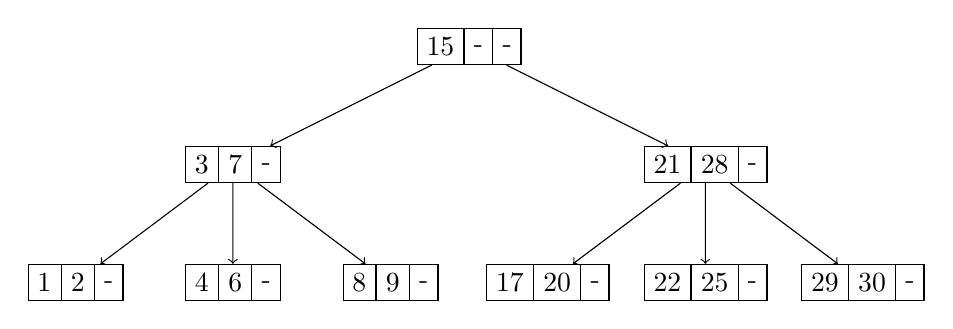
\begin{tikzpicture}
\tikzstyle{bplus}=[rectangle split, rectangle split horizontal,rectangle split ignore empty parts,draw]
\tikzstyle{every node}=[bplus]
\tikzstyle{level 1}=[sibling distance=60mm]
\tikzstyle{level 2}=[sibling distance=20mm]
\node {15 \nodepart{two} - \nodepart{three} - } [->]
  child {node {3 \nodepart{two} 7 \nodepart{three} - }
    child {node {1 \nodepart{two} 2 \nodepart{three} -}}
    child {node {4 \nodepart{two} 6 \nodepart{three} -}}
    child {node {8 \nodepart{two} 9 \nodepart{three} -}    }
  } 
  child {node {21 \nodepart{two} 28 \nodepart{three} -}
   child {node {17 \nodepart{two} 20 \nodepart{three} -}}
    child {node {22 \nodepart{two} 25 \nodepart{three} -}}
    child {node {29 \nodepart{two} 30 \nodepart{three} -} }   
    }
;\end{tikzpicture}


\minmeth{Einfügen:} Suche; Wenn Blatt nicht voll: füge ein (sortierung beachten) \\
Wenn Blatt voll: (ggf. rekursiv)

\halfpage{
\begin{enumerate}
\item  Suche das mittlere Element $M_{itte}$, die elemente rechts davon kommen in ein neues Blatt;
\item  füge $M_{itte}$ in den Vater Knoten ein, der rechte Verweis zeigt auf das neue Blatt; 
\item füge das neue Element ein
\end{enumerate}   }

\minmeth{Löschen} 

\halfpage{
\begin{enumerate}
\item Element nicht in einem Blatt => tausche es mit dem Nachfolger in der Sortierreihenfolge; Anschließend löschen; 
\item ist die Seite danach zu Klein ($<\mincontent$) versuche Ausgleich mit direkten Nachbarblatt:
das dazwischenliegende Element x wird aus Vaterknoten in den zu kleinen Knoten verschoben, der Nachfolger/Vorgänger aus dem anderen Knoten an seine Stelle eingefügt, sein Verweis kommt an die leere Adresse vor/nach x.
\item Ist das nicht möglich: Füge 2 benachbarte Knoten + x aus Vaterknoten zu einem Zusammen. Wiederhole ggf. rekursiv.
\end{enumerate}}

\minmeth{B*-Baum} 
Beim Einfügen in volle Seite wird wie beim löschen zuerst versucht mit direkten Nachbarn auszugleichen => bessere Speicherausnutzung, geringere Höhe

\minmeth{B+-Baum}
Bei Datenbank-Indexen: nur die Schlüssel in B-Baum, Blätter zeigen auf die Datenblöcke, diese sind doppelt verkettet. Der Baum selbst enthält nur Schlüsselwerte
\newpage


\minpurp{Suche im Array}
\minmeth{Sequentiell}
gehe der reihe nach alle elemente durch bis das element gefunden \textbf{O(n)}

\minmeth{Binär}
Sortiertes Array; betrachte mittleres Element; \\
<: Wiederhole im linken Teilarray, >: im rechten; worst-Case: \textbf{ $O(\log_2n)$}

\minmeth{Quick-Select}
Suche k. kleinstes element: Analog zu probab. Quicksort, betrachte nur das Teilarray, in dem der Index k liegt;  durchschnitt \textbf{O(n)}

\minpurp{Selection-Sort}
Suche Minimum; Tausche es mit dem ersten Element; Wiederhole im Array [2...n], \textbf{ O\{$n^2$\}}

\minpurp{Bubble-Sort}
durchlaufe elemente, tausche mit nachfolger wenn dieser größer; wiederhole \textbf{O\{$n^2$\}}

\minpurp{Quicksort}
\halfpage{\begin{enumerate}
\item Wähle Pivot= letztes Element
\item lasse zeiger von beiden Enden des Restarrays nach innen laufen: \\
 wenn der rechte zeiger auf ein kleineres bzw. der linke auf ein größeres Element als das Pivot zeigt stoppe den zeiger; wenn beide gestoppt: tausche sie, wenn sich die Zeiger treffen tausche das Pivot nach innen 
\item Wiederhole Quicksort im Rechten und linken Teilarray.
\end{enumerate}
}
Laufzeit: best Case:$O(n\log_2n)$, worst-Case $O(n^2)$

\submeth{probabilistisch:} start: wähle zufälliges Element als Pivot und tausche ans ende
\quarterpage{
\minpurp{Heapsort}
Interpretation Array als binärer Heap;\\
a[2i] und a[2i+1] sind die Kinder von a[i];\\
 Array durchläuft die Ebenen von oben nach unten, von links nach rechts

Heapbedingung: Vater $\leq$ Kinder
}
\quarterpage{
z.B. $[\underbrace{37}, \underbrace{45,57}, \underbrace{59,58, 99}] $=\\
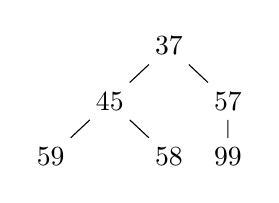
\begin{tikzpicture}[level distance=2em]
\node{37} 
child{ node{45}
child{ node{59}}
child{ node{58}}}
child{ node{57}
child{ node{99}}
}
;
\end{tikzpicture}
}

\minmeth{Heapsort}
Erzeuge Heap; 
Tausche letztes Element mit Wurzel, DownHeap in [1...n-1] , wiederhole bis array leer; 
worst-case: $O(n\log_2n)$

\minmeth{Erzeuge Heap}
Führe Einsichern für alle knoten durch (ebenenweise von unten rechts zur wurzel); \textbf{O(n)}

\minmeth{DownHeap}
Knoten > Kind: Tausche mit Kleinerem nachfolger; wiederhole rekursiv

\minmeth{Revisited}
Bestimme Pfad der kleineren Nachfolger bis zum Blatt, speichere den index.\\ 
=> index des i. Knotens auf dem Pfad sind die vordersten i Bits des Blattindex

\submeth{Lineare Suche:}
Suche vom Pfadende aus die Einfügestelle, speichere Wurzel, alle Pfadelemente rücken eine Ebene nach oben, einfügen Wurzel

\submeth{binärsuche:} analog dazu, suche Einfügestelle mit binärer Suche im Pfad 




\newpage

\minpurp{Netzwerk}
Quelle \textbf{S}, Ziel \textbf{T}

Flusserhaltung: für alle außer Quelle/Ziel: IN = OUT

Totaler Fluss: output(quelle) - input(quelle)


\minmeth{Ford Fulkerson (maximaler Fluss/Schnitt minimaler Kapazität)} Bilde Restgraph aus Netzwerk

\begin{minipage}{0.23\textwidth}
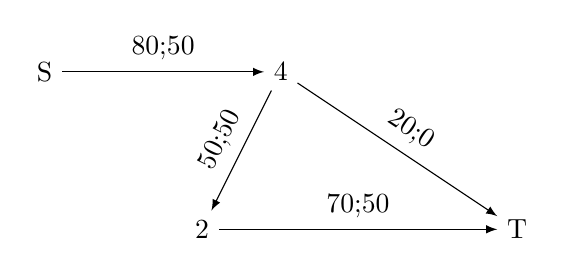
\begin{tikzpicture}[->,>=latex]
\tikzset{EdgeStyle/.append style = {->,bend left =20,black}}
\node(1)  at (0,2) {S}; \node(2) at (2,0){2}; \node(3) at (6,0){T};
\node(4) at (3,2){4};
\draw[->] (2) -> (3) node [above=0.25mm, midway,sloped] {70;50};
\draw[->] (1) -> (4) node [above=0.25mm, midway,sloped] {80;50};
\draw[->] (4) -> (3) node [above=0.25mm, midway,sloped] {20;0};
\draw[->] (4) -> (2) node [above=0.25mm,midway,sloped] {50;50};
\end{tikzpicture}
\end{minipage}$\Rightarrow$
\quarterpage{
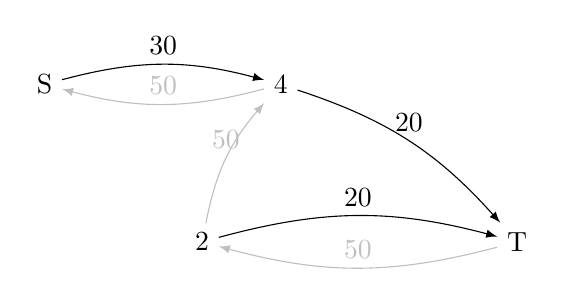
\begin{tikzpicture}[->,>=latex]
\node(1)  at (0,2) {S}; \node(2) at (2,0){2}; \node(3) at (6,0){T};
\node(4) at (3,2){4};
\path (1) edge [above=0.25mm,bend left=15] node  {30} (4);
\path (4) edge [above=0.25mm,bend left=15] node  {20} (3) edge [above=0.25mm,bend left=15,lightgray] node  {50} (1);

\path (2) edge [above=0.25mm,bend left=15, lightgray] node  {50} (4) ;

\path (3) edge [above=0.25mm,bend left=15,lightgray] node  {50} (2);
\path (2) edge [above=0.25mm,bend left=15] node  {20} (3);
\end{tikzpicture}}

Suche Pfad von Quelle -> Ziel, erhöhe fluss an diesem Pfad um dessen minimale Kante\\
Wiederhole solange ein Pfad Quelle -> Ziel existiert

\submeth{Edmonds-Karp} wähle den Pfad im Restgraph mit wenigsten \textbf{Kanten} (durch Weitensuche von der Quelle aus) $\mathbf{O(ke^2)}$\\
\submeth{Schnitt minimaler Kapazität: } Zusammenhangskomponente von S im Restgraph nach Ford-Fulkerson)~\\\\\\
\minpurp{Priority Queue}
Speichert Elemente mit Prioritäten, entnahme des Elements mit kleinster Priorität;
 
Implementierung durch Heap und Positionsarray für die Elemente;

Wird durch UpHeap/DownHeap die Position verändert: anpassen des Positionsarrays

\minmeth{Einfügen} füge das Element am HeapEnde ein, Umgekehrtes DownHeap (UpHeap) \\
\minmeth{Löschen} Entnahme der Heapwurzel, ersetzen durch letztes Element; DownHeap

\minpurp{Union-Find}
dynamische Partitionierung; parent array; Für Erweiterungen: array rank\\
Partition als Wurzelbaum => Elemente in einer Menge wenn gleiche Wurzel\\
Repräsentant ist Wurzel; Wurzeln haben parent[w] =0

\minmeth{Find(e)}
return Wurzel der Partition von e : durchlaufe parent-Beziehung bis Wurzel\\
\submeth{Pfadkomprimierung:} setze gefundene Wurzel als parent aller Knoten auf diesem Pfad 

\minmeth{Union(x,y)}
return true wenn in selber Partition, sonst false + vereinige diese Partitionen\\
i = Find(i); j = Find(j) if(i!=j) \{ parent[i] = Find(j)\}\\
\submeth{Höhen-Balancierung} rank[i] speichert rang von i; hänge bei Union die Kleinere Wurzel unter die größere, bei gleichheit steigt der rang der neuen Wurzel

worst-case Laufzeit für n-1 unions und m finds: \textbf{O((m+n)$\alpha(n));~~~ \alpha(n) \leq 4$}






\newpage
\minpurp{Graphen}
\textbf{k = Anzahl Knoten, e = Anzahl Kanten}

a adjazent zu b: es existiert die kante a->b, also $(a,b) \in E$\\
\submeth{Umgebung:} alle zu einem knoten adjazenten knoten

$e \leq \left( \! \begin{array}{c}k \\ 2\end{array} \! \right)$ (ungerichtet) bzw. $\leq k(k-1)$(gerichtet)

%vollständig: alle Kanten im Graph

%dicht/dünn besetzt: Anzahl der Kanten groß/klein im Vergleich zu möglichen kanten

\submeth{Teilgraph:} Knoten und Kanten sind Teilmenge des Originalgraphen\\
\submeth{aufspannender Teilgraph:} alle Knoten und Teilmenge der Kanten des Originalgraphen\\
\submeth{erzeugender Teilgraph:} Teilmenge der Knoten und alle Kanten zwischen diesen

\submeth{Pfad:} Folge von Knoten $v_0,v_1,\dots,v_n$, mit Kanten von $v_i -> v_{i+1}$\\
%einfacher Pfad: jeder Knoten nur einmal im pfad\\
%geschlossen: Anfang = Ende des Pfads\\
\submeth{Zyklus:} geschlossener Pfad mit länge $\geq$ 3 (ungerichtet) bzw. $\geq$ 2 (gerichtet)

\submeth{Zusammenhangskomponente:} alle gegenseitig erreichbaren knoten bilden Komponente\\
\submeth{Baum:} zusammenhängend, azyklisch und e = k-1\\
\submeth{Bipartiter Graph:} zwei Mengen von Knoten $V_1, V_2$, alle Kanten gehen von $V_1$ nach $V_2$
%\textcolor{lightgray}{perfekte Zuordnung: Bipartiter Graph, bijektive Abbildung von $V_1$ nach $V_2 \Leftrightarrow$ det(Adjazenzmatrix) = 0}

Adjazenzmatrix: $\left(
\begin{matrix}
0 & 1& 0\\
0 & 0 & 0 \\
1 & 0 & 0 
\end{matrix}
 \right)$ => 
\tikzset{ LabelStyle/.style = { rectangle, rounded corners, draw, minimum width = 2em, font =fseries }, VertexStyle/.append style = { inner sep=5pt, font = \Large\bfseries}, EdgeStyle/.append style = {->,bend left =20}}
\begin{minipage}{0.1\textwidth}
\begin{tikzpicture}
\tikzset{EdgeStyle/.append style = {->,bend left =20,black}}
\node(1){1}; \node(2)[above right of=1]{2}; \node(3)[below right of=2]{3};
\draw[->] (1) edge (2) (3) edge (1);
\end{tikzpicture}
\end{minipage}
Adjazenzliste: 
\begin{minipage}[c]{0.1\textwidth}
1: 2\\
2:\\
3: 1 \\
\end{minipage}.

\minpurp{Weitensuche}
Besuche die Nachbarn des Startknotens, dann die Nachbarn des ersten Nachbarn usw.\\
$\Leftrightarrow$ gehe den entstehenden Baum Ebenenweise durch.

$V_T:$ besuchte Knoten, $V_{ad}$: zum besuch Vorgemerkte Knoten als Queue, $V_R$: Rest

\textcolor{lightgray}{Ablauf: int[k] where; // <0: in der Queue, 0: $V_R$, >0: besucht }%(nummer gibt die Zusammenhangskomponente an);

Visit(Node k): füge k in die Queue;\\
durchlaufe die Queue, für jeden Knoten füge alle Nachbarn aus $V_R$ in die Queue

Laufzeit: bei Liste:\textbf{ O(e+k)}, bei Matrix: $\mathbf{O(k^2)}$

\minmeth{Erweiterung:} Test auf Zyklen $\Leftrightarrow$ Test ob Nachbar schon im Baum (und nicht parent)\\
Ermittlung des Abstands von der Wurzel des erzeugten Baums

\minpurp{Tiefensuche}
Besuche den 1.Nachbarn des Startknotens, dann den 1.Nachbarn des 1.Nachbarn usw.\\
$\Leftrightarrow$ durchlaufe einen Pfad nach dem Anderen

Visit: durchlaufe die Adjazenzliste, für jeden nicht besuchten nachbarn rufe Visit auf\\
Laufzeit: \textbf{O(e+k)}


\minmeth{Erweiterung:} 
\submeth{Test auf Azyklität} Kanten auf einen Vorgänger\\
bei Visit Start/Ende: A vorgänger von B wenn $[Start_B,End_B] \subset  [Start_A,End_A]$

\submeth{Topologisches Sortieren} Array der Länge k, fülle von hinten bei Visitende\\
\submeth{Starke Zusammenhangskomponente:}

\halfpage{
\begin{enumerate}
\item Nummeriere in Terminierunsreihenfolge
\item Drehe alle Kanten um ( Konstruiere den reversen Graph)  
\item Tiefensuche von höchster Terminierungsnummer aus, alle Erreichbaren sind starke Zusammenhangskomp. 
\item(wiederhole letzten Schritt bei bedarf)
\end{enumerate}
}

\minpurp{Priority Queue}
Speichert Elemente mit Prioritäten, entnahme des Elements mit kleinster Priorität;
 
Implementierung durch Heap und Positionsarray für die Elemente;

Wird durch UpHeap/DownHeap die Position verändert: anpassen des Positionsarrays

\minmeth{Einfügen} füge das Element am HeapEnde ein, Umgekehrtes DownHeap (UpHeap) \\
\minmeth{Löschen} Entnahme der Heapwurzel, ersetzen durch letztes Element; DownHeap

\minpurp{Union-Find}
dynamische Partitionierung; parent array; Für Erweiterungen: array rank\\
Partition als Wurzelbaum => Elemente in einer Menge wenn gleiche Wurzel\\
Repräsentant ist Wurzel; Wurzeln haben parent[w] =0

\minmeth{Find(e)}
return Wurzel der Partition von e : durchlaufe parent-Beziehung bis Wurzel\\
\submeth{Pfadkomprimierung:} setze gefundene Wurzel als parent aller Knoten auf diesem Pfad 

\minmeth{Union(x,y)}
return true wenn in selber Partition, sonst false + vereinige diese Partitionen\\
i = Find(i); j = Find(j) if(i!=j) \{ parent[i] = Find(j)\}\\
\submeth{Höhen-Balancierung} rank[i] speichert rang von i; hänge bei Union die Kleinere Wurzel unter die größere, bei gleichheit steigt der rang der neuen Wurzel

worst-case Laufzeit für n-1 unions und m finds: O((m+n)$\alpha(n));~~~ \alpha(n) \leq 4$

\minpurp{Dijkstra/Prim (minimaler aufspannender Baum)}
\submeth{Start:} (\{Startknoten\}, $\emptyset$) ~~~~// Startknoten, keine Kanten\\
\submeth{Schritt:} füge die kleinste vom konstruierten Baum ausgehende Kante in den baum ein;\\
Priorität: bei Prim: Kantengewicht, bei Dijkstra Pfad zur Wurzel\\
Implementierung durch Priority Queue bei Adjazenzliste

Laufzeit: \textbf{O($n^2$)} bei Matrix, \textbf{O((p+q)log(p))} bei liste

\minpurp{Kruskal (minimaler aufspannender Baum)}
\submeth{Start} T= (V,$\emptyset$) ~~~~// alle Knoten, keine Kanten\\
\submeth{Schritt} füge die kleinste Kante ein, die keinen Zyklus erzeugt\\
Implementierung: Knoten in Union-Find; Sortiere Kanten nach gewicht, durchlaufe die Kanten und führe für jede Kante Union($v_{Start},v_{End}$) aus; wenn false füge die Kante ein;\\
Laufzeit: O(p+qlog(q))

\minpurp{Boruvka (minimaler aufspannender Baum)}
Min-Max-Ordnung: kante ist Kleiner falls gewicht kleiner bzw. kleinerer Knoten kleiner bzw. größerer Knoten kleiner\\
minimale indizente Kante: kleinste Kante an einem Knoten\\
\submeth{Start:} Tree(V,$\emptyset$) Graph(V,E)\\
\submeth{Schritt:} füge alle Minimal indizenten Kanten im Baum ein, Kontrahiere sie im Graph; wiederholen
Laufzeit: \textbf{O((p+q)log(p))}

\minpurp{Warshall (transitiver Abschluss)}
Erzeugt Graph, bei dem jede Kante einem Pfad in der Eingabe darstellt


\submeth{Start:} $a_0$ = Adjazenzmatrix;

für k=1 bis p: 

\submeth{Schritt:} $a_k[i,j] = a_{k-1} or( a_{k-1}[i,k] and a_{k-1}[k,j] )$
für implementierung: es wird nur speicher für eine Matrix benötigt, diese wird angepasst. 3 forschleifen (k,i,j) => 
\textbf{O($p^3$)}

\minpurp{Floyd (minimaler aufspannender Baum)}
Adjazenzmatrix gewichteter Graph, gewicht= $\infty$ wenn keine Kante, 0 in Hauptdiagonale;

\submeth{Start:} $a_0$ = Adjazenzmatrix;

für k=1 bis p: 

\submeth{Schritt:} Schritt: $a_k[i,j] = min{a_{k-1} , a_{k-1}[i,k] + a_{k-1}[k,j] }$

funktioniert auch mit negativen gewichten, wenn keine negativen Zyklen, implementierung analog zu Warshall



\end{document}